\section{Method}


\subsection{Trajectory Representation}

The final goal of our optimization is to compute three trajectories:
radiation dose-rate $r(t)$, lower leaf position $z_L(t)$, and upper leaf position $z_U(t)$.
Each of these trajectories is represented by a piecewise linear spline,
with shared knot times $t_k \in \{t_0, t_1, \dots, t_N\}$, where $N$ is the number of knot points.
The value of the dose rate and leaf positions at knot time $t_k$ are given by
$r_k$, $x_{L,k}$, and $y_{U,k}$ respectively.

\begin{figure}
  \centering
  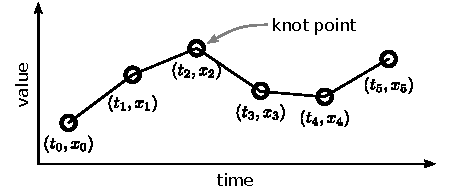
\includegraphics{fig/linearSpline.pdf}
  \caption{Linear Spline. We represent the dose-rate and leaf position trajectories as linear
           splines. A linear spline is fully defined by its value at the knot points. }
  \label{fig:linearSpline}
\end{figure}

\subsection{Trajectory Limits}

There are several constraints imposed on the dose-rate and leaf trajectories
by the physical limitations of the VMAT machine. Specifically, there is a maximum dose-rate,
constant limits on the leaf positions, and an upper limit on the leaf speed.
These limits are detailed below, where $\dot{z}(t) = \tfrac{d}{dt}z(t)$ gives the leaf velocity.
\begin{align}
  \text{dose-rate: }& \quad 0 \leq r(t) \leq r_\text{max}
      \label{eqn:FirstTrajectoryConstraint}\\
  \text{leaf position: }& \quad x_{min} \leq z_L(t) \leq z_U(t) \leq x_\text{max} \\
  \text{lower leaf velocity: }& \quad v_\text{min} \leq \dot{z}_L(t) \leq v_\text{max} \\
  \text{upper leaf velocity: }& \quad v_\text{min} \leq \dot{z}_U(t) \leq v_\text{max}
      \label{eqn:LastTrajectoryConstraint}
\end{align}

\subsection{Avoiding Local Minima}

One of the key issues with fluence mapping is that the
optimization tends to get stuck in local minima,
since there are a large number of leaf trajectories that deliver the same fluence to the target.
\addref{local minima in fluence mapping}
Of these many solutions, the most desirable solutions are those which have smooth leaf trajectories,
because they reduce wear on the machine and less likely to exploit inaccuracies in the model.
\MPKcomment{Need some reference here, or perhaps a better explanation of why smooth is good.}
One way to create a smooth trajectory is to minimize the integral of the derivative-squared,
a regularization trick that is commonly used in trajectory optimization of dynamical systems.
\addref{torque-squared optimization}
For our problem, this regularization term can be written:
\begin{equation}
  J_\text{vel}\big(\dot{z}_L(t), \dot{z}_U(t)\big)
    = \int_0^T \! \big( \dot{z}_L^2(t) + \dot{z}_U^2(t) \big) \,dt
\end{equation}

\subsection{Computing Delivered Fluence}

The fluence delivered at each position on the target is computed by integrating the
dose-rate function over the periods of time when the leaves are not blocking the target:

\begin{equation}
  f_D(x) = \int_{\mathcal{T}(x)} \! r(t) \,dt
  \quad \quad
  \mathcal{T}(x) = \forall t
  \quad
  \text{S.T.}
  \quad
  z_L(t) \leq x \leq z_U(t)
  \label{eqn:fluenceMapIntegral}
\end{equation}
\MPKcomment{Is there a better way to write the definition of $\mathcal{T}$?}

It is tricky to compute this integral directly, as it would require computing
the inverse of the leaf trajectories.
In addition, it creates a discontinuity in the gradient
(\textit{e.g.} $\tfrac{\partial f_D}{\partial z_L})$)
which can cause issues when putting this integral inside of an objective function.

Our solution is to rewrite the integral using a blocking function $k(t)$,
which has a value of one when the leaves are passing radiation and
zero when the leaves are blocking radiation, as described in \S\ref{sec:modelingFluenceBlocking}
This allows us to rewrite (\ref{eqn:fluenceMapIntegral}) using the bounds $[0, \mathcal{T}]$:

\begin{equation}
  f_D(x) = \int_0^T \! k(t, x) \cdot r(t) \, dt
  \label{eqn:fluenceDoseSimpleBounds}
\end{equation}

Now we have a standard scalar integral, where the integrand is smooth and the
bounds are constant, we can use any quadrature method to evaluate (\ref{eqn:fluenceDoseSimpleBounds}).
In this case we use the trapezoid rule with a dense grid spacing.

\subsection{Modeling Fluence Blocking}
\label{sec:modelingFluenceBlocking}

A simple way to define the fluence blocking function $k(t)$
would be to set it to one if $z_L(t) \leq x \leq z_U(t)$
is true, and zero otherwise.
This implementation would have a discontinuous gradient, which would cause problems in the optimization.
Instead, we use a polynomial smoothing to approximate the step function $s(x,\alpha)$,
where $\alpha$ is a smoothing parameter.
Note that the function $s(x,\alpha)$ has continuous value, slope, and curvature.

\begin{equation}
  k(t, x) = s\big(x - z_L(t), \alpha\big) \; \cdot \; s\big(z_U(t) - z, \alpha\big)
\end{equation}

\begin{equation}
  s(x, \alpha) =
    \begin{cases}
      0, & \text{for } x \leq -\alpha \\
      6\tau^5-15\tau^4+10\tau^3, & \text{for }  -\alpha < x < \alpha\\
      1, & \text{for } x \geq \alpha
    \end{cases}
\end{equation}

\begin{equation}
  \tau(x) = \frac{x + \alpha}{2\alpha}
\end{equation}

\subsection{Objective Function}

The objective function for the inner optimization (computing leaf trajectories)
is a weighted combination between the fitting error and the smoothing regularizaiton.
The fluence fitting objective is the integral of the squared-error
between the target fluence $f_T(x)$ and the delivered fluence $f_D(x)$.

\begin{equation}
  J_\text{fit} = \int_{x_{min}}^{x_{max}} \! \big( f_T(x) - f_D(x) \big)^2 \,dx
\end{equation}

Like the other integrals, we evaluate this integral using the trapezoid rule,
although the specific choice of quadrature method is not important.

The final objective function is a weighted combination of the
fitting objective $J_\text{fit}$ and the smoothing objective $J_\text{vel}$.
Since the fitting objective is an integral over position, and the smoothing objective
is computed over time, we normalize both before combining.

\begin{equation}
  J = \frac{1}{(x_{max} - x_{min})} J_\text{fit}
    + \frac{\beta}{T} J_\text{vel}
\label{eqn:FluenceFittingObjective}
\end{equation}

\subsection{Transcription to a Nonlinear Program}

The inner optimization loop computes the leaf trajectories ($z_L(t), z_U(t)$)
that minimize the objective function (\ref{eqn:FluenceFittingObjective})
and satisfy the constraints (\ref{eqn:FirstTrajectoryConstraint}--\ref{eqn:LastTrajectoryConstraint}).

Since we represent the position trajectories $z_L(t)$ and $z_U(t)$ as piecewise linear,
it is natural to represent them by their values at the knot points $t_i$.
The position trajectory is piecewise linear, thus it follows that we should represent the
velocity trajectory as piecewise constant.
Here we will use a direct collocation transcription method, where the velocity for the
lower $v_L$ and upper $v_U$ leaves are decision variables.
is a decision variable in the optimization,
and we add a constraint to ensure that the velocity is the derivative of position.
This is done to keep the gradients in the optimization sparse \ref{Betts2010}.
We with our quadrature calculations, we will use trapezoidal quadrature for the integral constraint.
We will define the segment duration $h_k = (t_{k+1} - t_k)$.

\begin{align}
  v_{L,k} & = \tfrac{1}{2} h_k \cdot  \big( z_{L, k} + z_{L, k+1} \big)
  \quad \quad \forall k\\
  v_{U,k} & = \tfrac{1}{2} h_k \cdot  \big( z_{U, k} + z_{U, k+1} \big)
  \quad \quad \forall k\\
\end{align}

The limits on leaf position and velocity can be implemented as a combination of
constant bounds and linear inequality constraints:

\begin{equation}
  x_\text{min} \leq x_{L, k}
  \quad \quad
  x_{U, k} \leq x_\text{max}
  \quad \quad
  x_{L, k} \leq x_{U, k}
  \quad \quad
  \forall k
\end{equation}

\begin{equation}
  v_\text{min} \leq v_{L,k} \leq v_\text{max}
  \quad \quad
  v_\text{min} \leq v_{U,k} \leq v_\text{max}
  \quad \quad \forall k
\end{equation}

\todo{Add a summary sentence about how to pack everything up into a NLP solver}
